\section{System Design} \label{section:coordinator}

\todo{ETK make sure 'publisher', 'subscriber', 'client' have all been defined by this point}
\todo{ETK if these goals are already outlined somewhere else then no need to put them here}

Our design is motivated by a number of goals that we wish to achieve:
\begin{itemize}
\item High Availability: We wish to create a system that is resilient in the face of arbitrary machine failures.
\item Scalability: The system should be able to scale to large numbers of clients with reasonably high message rates.
\item Simple Clients: The code necessary for a client to interact with the system should be very simple, since we assume that they may be embedded devices with limited programming facilities.
\end{itemize}

\subsection{Overview}

\begin{figure*}[t]
\centering
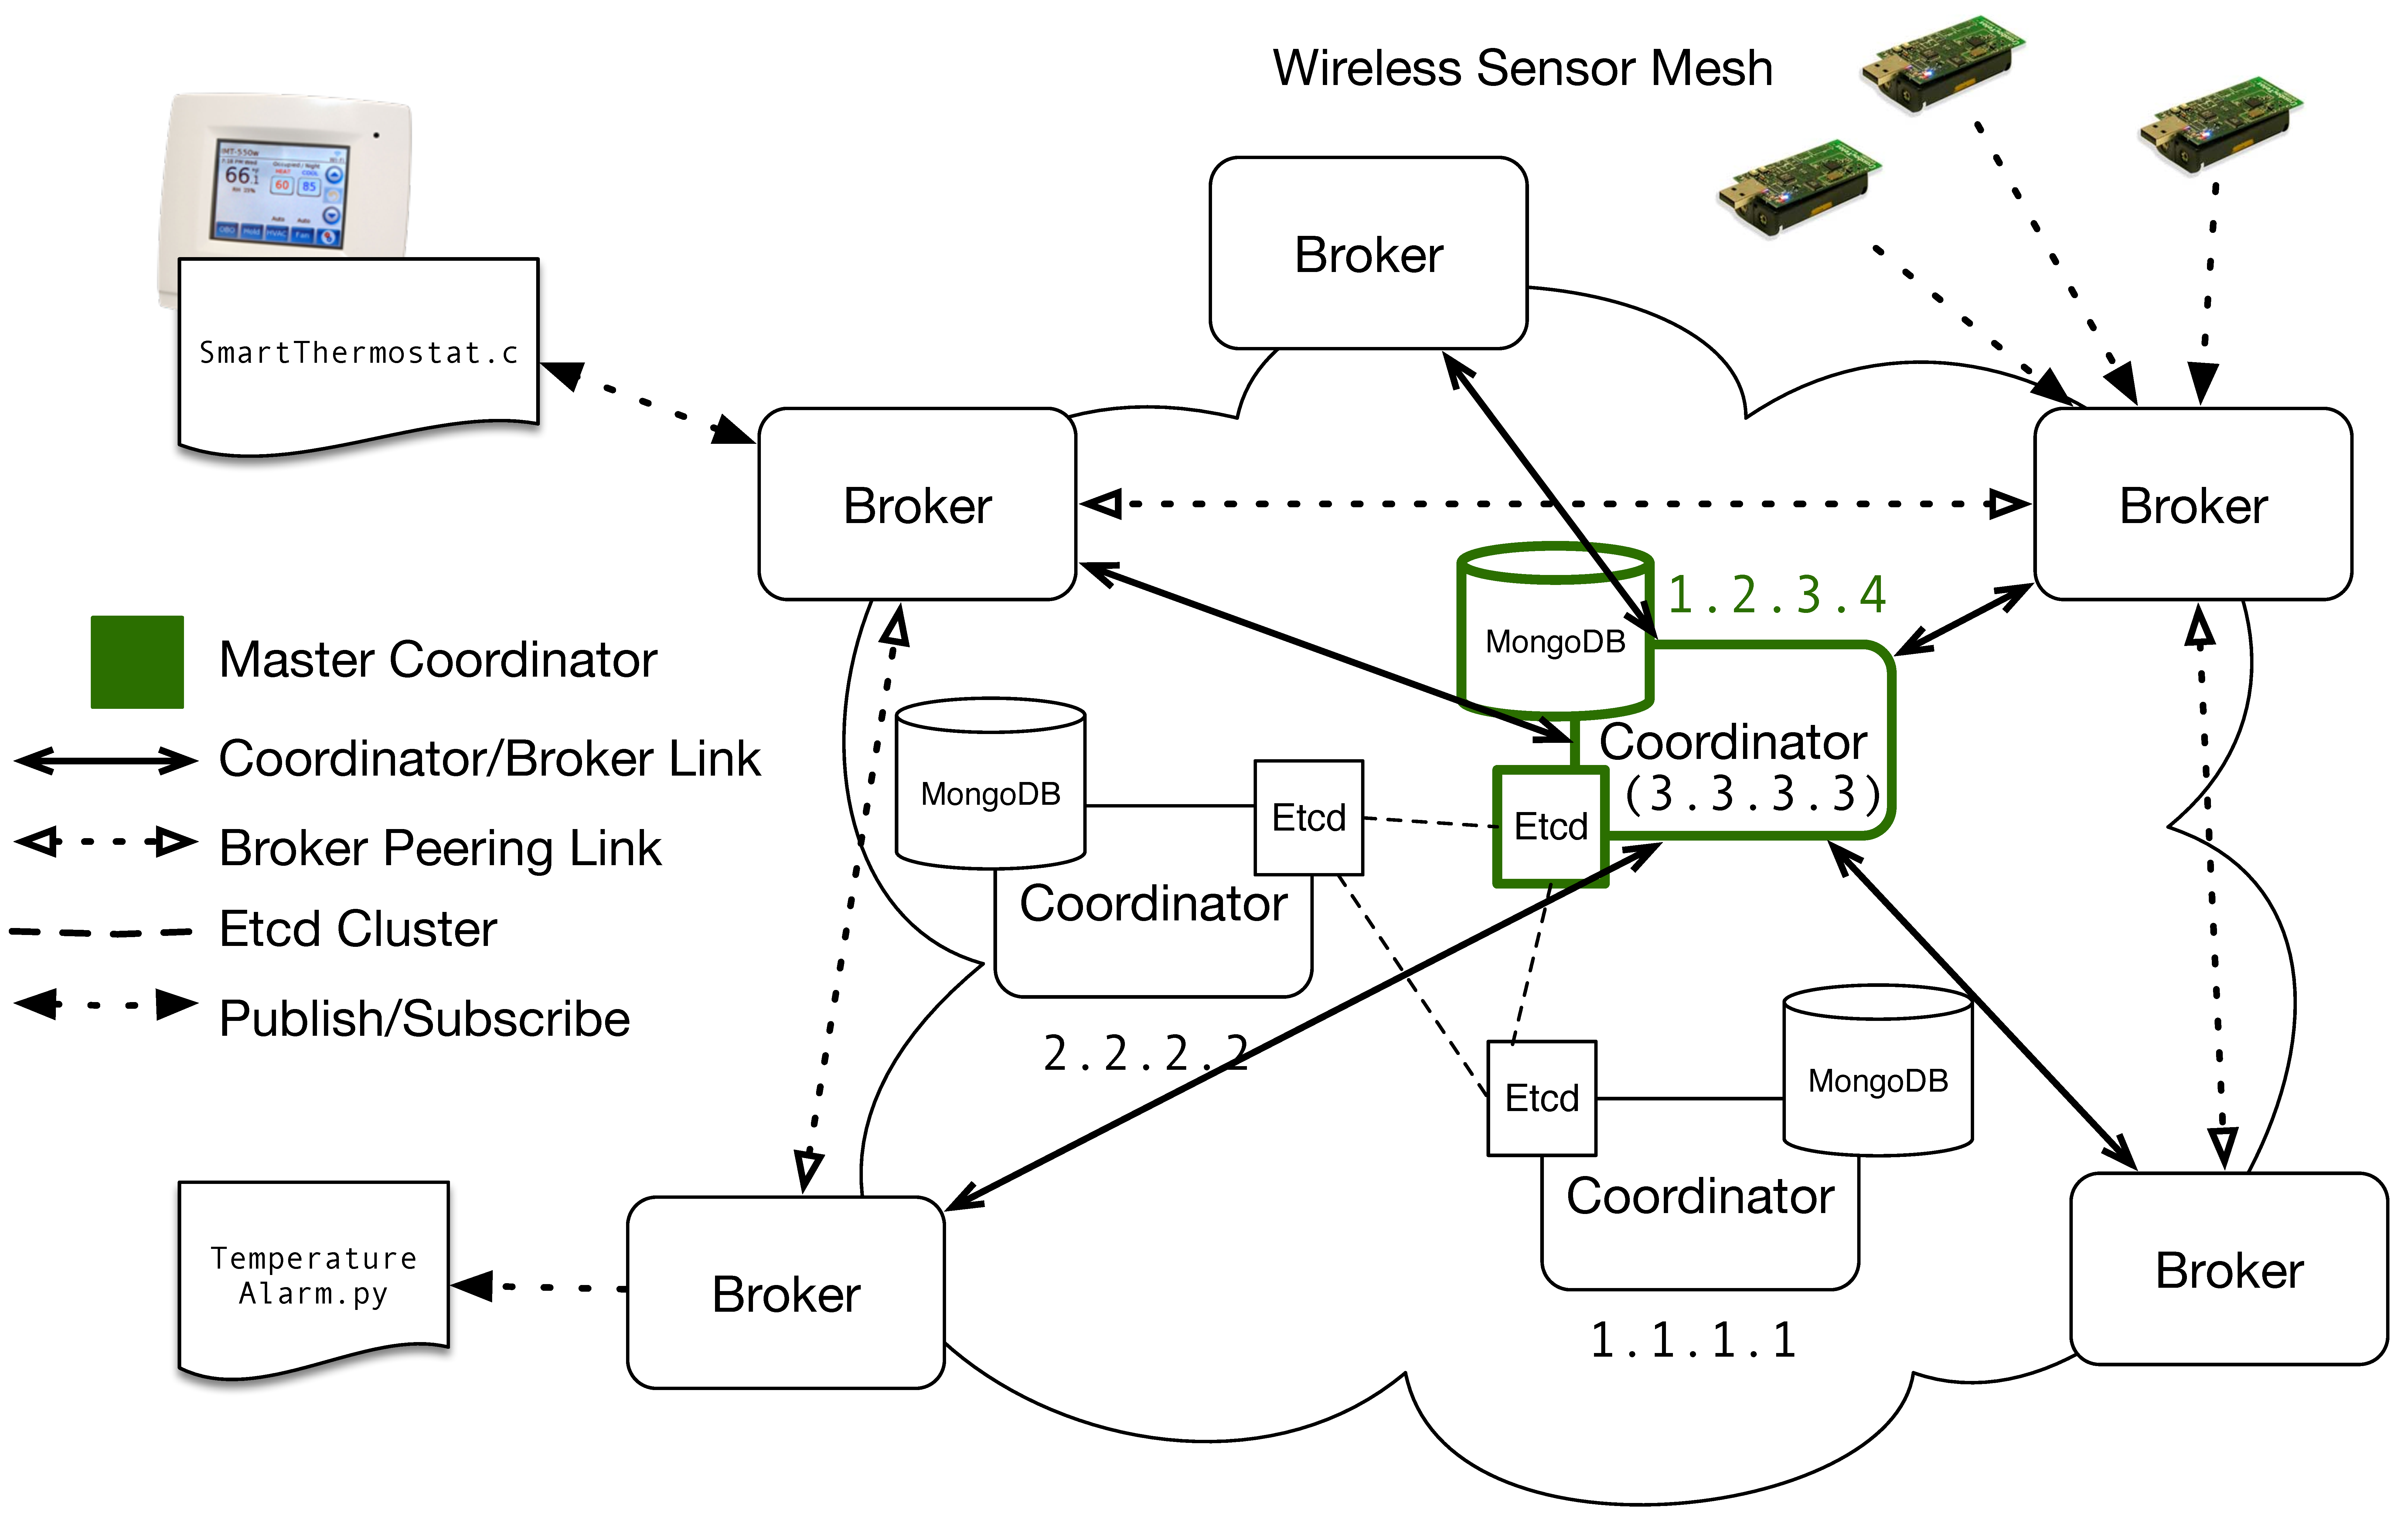
\includegraphics[width=6.5in]{figs/full_architecture.pdf}
\caption{Overview of the architecture of our brokerage system.
Numerous clients communicate to a set of decentralized brokers which create a forwarding network between themselves as instructed by the centralized coordinator nodes.}
\label{fig:architecture}
\end{figure*}

To meet these goals, we have developed an architecture which consists of two primary components: distributed brokers and centralized coordinators.
See Figure~\ref{fig:architecture} for an overview which will be described in more detail in this and the following sections.

The system contains one logically centralized coordinator; to all other entities in the system, the coordinator can be treated as a single machine.
In actuality, this logical coordinator consists of three independent nodes to improve fault tolerance; see Section~\ref{subsec:coordinator_fault_tolerance} for more detail.
This coordinator makes all of the decisions in the system, determining when a broker has failed, which brokers should forward which messages where, when changes occur to the set of publishers a subscriber is currently receiving messages from, which broker a client should contact if their broker fails, etc.
It then distributes these decisions to the brokers, which take appropriate action.
To do this the coordinator stores the current state of all brokers in the system, as well as information about all of the clients that are known to the system, i.e.\ what broker they are attached to, what query they are interested in (for subscribers), and what their current metadata is (for publishers).
Publisher metadata is stored in a local instance of MongoDB\footnote{\url{https://www.mongodb.com/}} which is used for executing queries.

Brokers are numerous and may reside anywhere; for example, a deployment may consist of a broker located in each building which contains client devices, or brokers may be run on cloud computing nodes.
Brokers are responsible for communicating with clients and for forwarding messages along routes as instructed by the coordinator.
Any changes to the set of clients connected to the broker, or to the metadata of a publisher connected to the broker, are communicated back to the coordinator for handling so that the coordinator always has an update-to-date view of the entire system state.

\subsection{Normal Operation}
\label{subsec:normal_operation}

In this section we describe the events which take place under normal operation, i.e.\ in the case that there are no failures within the system.

\textbf{A new subscriber enters the system.}
A subscriber contacts its local broker, Broker A, whose address can be hardcoded into the client or discovered through some network discovery protocol, e.g.\ \todo{Gabe can you help here}
The subscriber submits a message to Broker A containing the query which defines which publishers' output it is subscribed to.
Broker A forwards the message along to the coordinator, which evaluates the query against the set of publisher metadata currently known to the system and replies to Broker A with the (possibly empty) set of relevant publishers.
If any relevant publishers are found, the coordinator will contact the broker at which they are located and instruct that broker to forward the publisher's messages to Broker A, which will in turn forward the messages to the subscriber.
We can see this, for example, in Figure~\ref{fig:architecture}: \texttt{SmartThermostat.c} is publishing to a broker which has a forwarding link established to another broker to which \texttt{TemperatureAlarm.py} is connected, establishing a publication route between \texttt{SmartThermostat.c} and \texttt{TemperatureAlarm.py}.

\textbf{A new publisher enters the system.}
A publisher contacts its local broker, Broker A, in the same manner as a new subscriber.
The publisher submits its initial set of key-value metadata pairs to Broker A, which forwards them to the coordinator.
The coordinator evaluates this new metadata against the set of currently active queries, notifies any subscribers whose queries apply to the new publisher, and constructs new forwarding routes from Broker A as in the previous case.

\textbf{A publisher submits new metadata.}
This process is essentially the same as adding a new publisher, except that in addition to possibly creating new forwarding links, some may need to be removed if the metadata changed in such a way that a publisher is no longer relevant to a subscriber's query.
Again, the coordinator will instruct Broker A about which brokers to create (and destroy) forwarding routes to.

\textbf{Clients leave the system.}
When subscribers and publishers leave the system, a similar process is followed; the coordinator is notified, and forwarding routes are created or destroyed as necessary.

\textbf{A publisher publishes a message.}
When a message does not contain any metadata changes, the coordinator is not involved in any part of the process.
The broker to which the publisher is connected simply broadcasts the message over all forwarding routes relevant to that publisher, and the recipient brokers will forward the message to the subscriber.

\subsection{Coordinator Fault-Tolerance}
\label{subsec:coordinator_fault_tolerance}

\begin{figure*}[t]
\centering
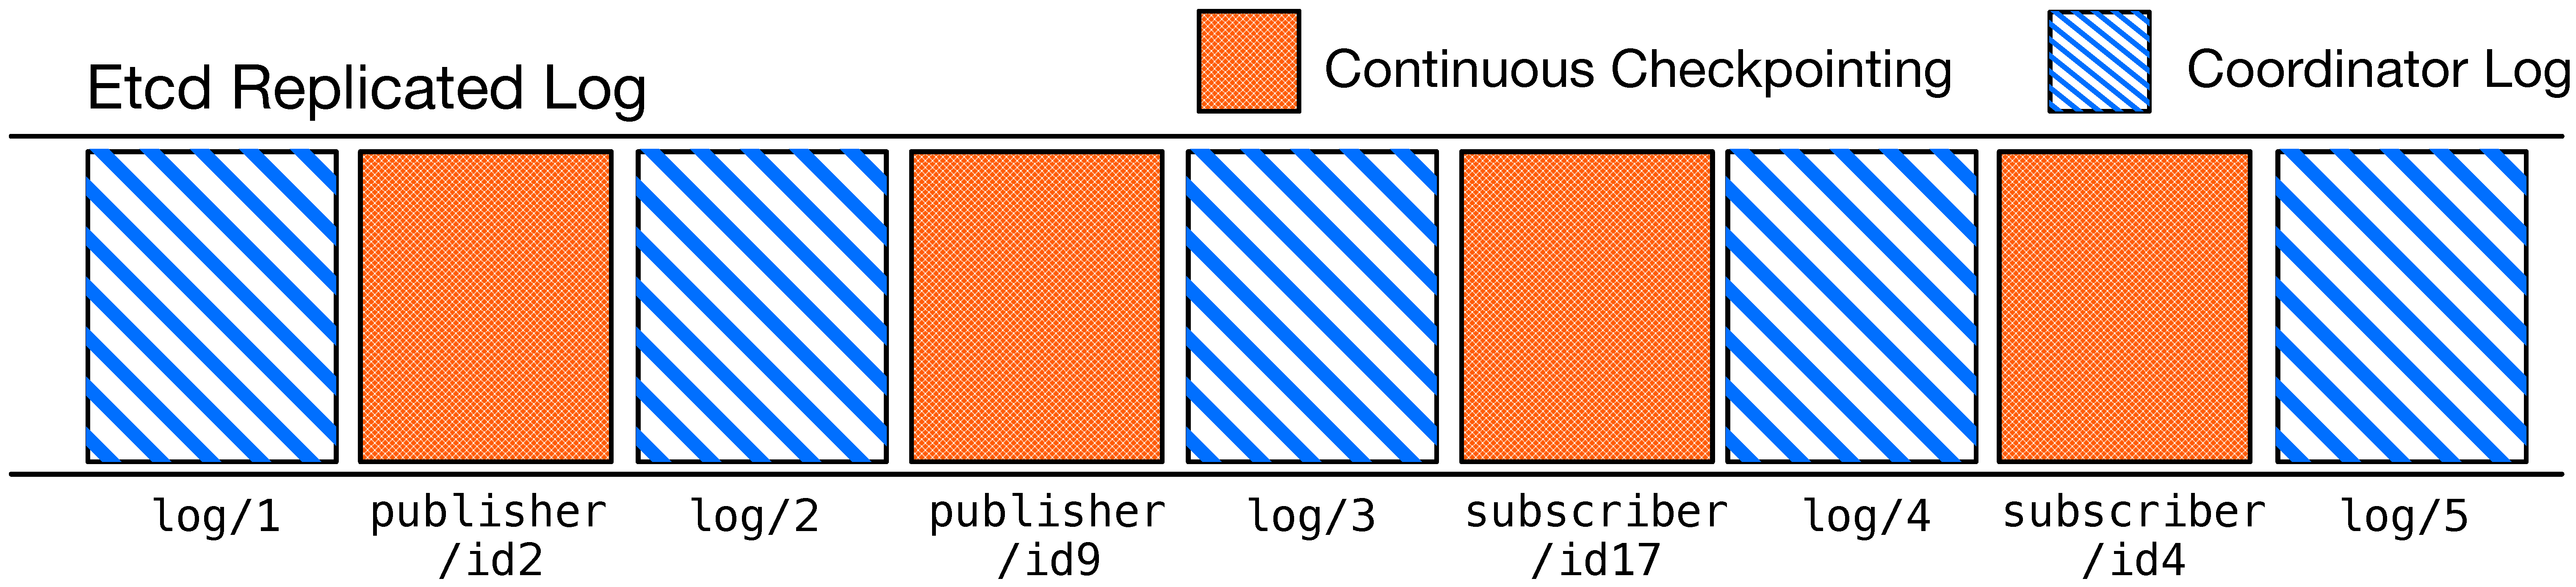
\includegraphics[width=.9\linewidth]{figs/logreplay.pdf}
\caption{Although they live in separate key spaces, the log and the continuous checkpointing are serialized via the Etcd log so that they can be leveraged for a consistent rebuild.}
\label{fig:logreplay}
\end{figure*}

To all other components of the system, including clients, the coordinator appears to be a single node which is resilient to failures; however, to construct a highly available system the coordinator must be able to handle at least one node failure.
To ensure that the coordinator will be resilient in the face of machine failure, we replicate its state across three independent nodes.
Each coordinator node runs an Etcd\footnote{\url{https://coreos.com/etcd/}} node, a reliable key-value store which internally uses the Raft distributed consensus protocol~\cite{ongaro2014} to provide strong consistency semantics among its members.
At any given time, one coordinator is designated as the leader; this is the only coordinator node which will accept messages from or send messages to brokers.
A single ``leader'' key is stored in Etcd; whichever coordinator was able to create this key via an atomic create-if-not-exists operation is considered the leader.
The key is marked with a time-to-live of a few seconds which is continually refreshed by the leader; if the leader fails to refresh its ownership of the key, the key will disappear, allowing another replica to become the new leader.

To make this cluster of machines with potential leadership changes appear to brokers and clients as a single machine, we maintain one external IP address at which the current leader can always be contacted (``1.2.3.4'' in Figure~\ref{fig:architecture}) in addition to the internal IP addresses which coordinators use to communicate with each other (``1.1.1.1'', ``2.2.2.2'', ``3.3.3.3'').
Various mechanisms can be used to ensure that this IP address always points to the correct coordinator; we run coordinator nodes on Amazon Web Services (AWS)~\footnote{\url{https://aws.amazon.com/}}, which provides an ``Elastic IP'' feature which allows for machine instances to request that an IP be reassigned to them.
Unfortunately the Elastic IP feature of AWS has delay of approximately 10--15 seconds (measured during our own experiments) before new requests are successfully routed to the correct host after the mapping has changed; this is a limitation of AWS and not fundamental to our protocol.

Every time a message is received from a broker, the leader logs the message to Etcd to make it durable before processing.
The replicas watch this log, continually applying log entries to their state as if they received the message from a broker.
This ensures that replicas are always very close to update-to-date with the state of the leader, lagging behind by only the latency of a write-read pair through Etcd (on the order of tens of milliseconds), making IP reassignment the only reason that coordinator failover is not extremely fast.
When the leader is finished processing a message, it sends an acknowledgment back to the originating broker.
If the broker does not receive an acknowledgment, it will resend the message.
So, if a leader writes a message to the log and crashes before finalizing its processing, the broker will eventually resend the message to the new leader, which ensures that the necessary operations are eventually completed.
Since messages are idempotent (e.g.\ attempting to create the same forwarding route twice has no effect the second time), it is acceptable for the new leader to redo some actions that the old leader carried out.

In addition to storing a log of inbound messages, the leader also stores the current state of each client and broker as a key-value pair within Etcd.
This is essentially a form of continuous checkpointing which enables a newly instantiated coordinator replica to quickly catch up to the state of the leader.
Rather than reading and executing the log from the beginning of time, a new replica can read the current state of the system via the client and broker keys up to some fixed point in time, then resume reading the log from that same point in time.
To maintain consistency between the continuous checkpoint and the log, we make use of the fact that Etcd internally maintains a sequential log of events (a consequence of using Raft).
Each modification to the Etcd store is marked with a revision number which indicates the order in which the modifications occurred.
By choosing some revision number and reading all client/broker state up to and including that revision, then reading all log entries after that revision, it is ensured that the replica switches from reading the checkpoint to reading the log in a consistent manner; see Figure~\ref{fig:logreplay}.
Note that this works even if the client or broker key was overwritten (i.e.\ if a change to the state occurred which was then written to Etcd) because Etcd stores versioned copies of key-value pairs.

To clear old checkpoint versions and unnecessary log entries, the leader periodically performs garbage collection.
Replicas periodically write the sequence number of the last log entry they have processed to a specific key in Etcd.
The leader periodically checks these values and instructs Etcd to delete entries which both replicas have already read, as well as instructing Etcd to perform a ``compaction'' up to this point, which removes old versions of keys which are no longer needed.

\subsection{Broker Fault-Tolerance}

In addition to being resilient to coordinator failures, we require that our system continue functioning and all clients continue to be able to participate in the face of a broker failure.
To this end, and with low client complexity in mind as a goal, we have designed a very simple fail-over protocol which allows the client to continue to operate on another broker during the period in which its local broker is not available.

In addition to being aware of its local broker as described in Section~\ref{subsec:normal_operation}, each client must know the external address of the coordinator.
First, a client attempts to contact its local broker, Broker A.
If the client is unable to do so, it sends a request to the coordinator, which will supply it with the address of some other broker B which can service its needs until Broker A is available again.
The client connects to Broker B and continues as usual.
When Broker A becomes available, the coordinator instructs Broker B to sever its connection to the client, which will then attempt to contact Broker A as usual. This can be summarized by the following pseudocode:

% TODO maybe could use some work
\begin{lstlisting}[language=pseudocode,basicstyle=\small]
while client_active:
  success := connect_to(local_broker_address)
  if success:
    // process ...
  else:
    broker_addr := connect_to_get_message(coordinator_address)
    success := connect_to(broker_addr)
    if not success:
      continue
    // process ...
\end{lstlisting}

\subsection{Design Discussion}

This design allows us to meet all of our goals.
We have high availability via fault tolerance for both broker and coordinator failures.
The necessary code for clients is very simple; publishers need to know how to send publication messages, subscribers need to know how to send query messages and receive publication messages and subscription difference messages (e.g.\ publisher A just became relevant to your query), and both need to know how to ask the coordinator for a fail-over broker.
We also have scalability in terms of number of messages that can be sent through the system by removing any coordination from the normal message forwarding path, which can be scaled arbitrarily with the number of brokers.

One aspect on which this design is lacking is that the coordinator is a bottleneck for changes to the state of the system (i.e.\ clients entering or leaving and publishers changing metadata).
We assume that in comparison to the rate of messages being sent in the system, changes to the set of connected clients and to the metadata associated with publishers is relatively slow, so we consider this design to be acceptable.
Part of the reason for choosing this design was its relative simplicity; we have considered two alternate designs which were considered and which we hope to evaluate as future work (see Section~\ref{subsec:alternate_designs})..

%%% Local Variables:
%%% mode: latex
%%% TeX-master: "paper"
%%% End:
